\documentclass{article}
\usepackage[margin=1.2in]{geometry}
\usepackage[T1]{fontenc}
\usepackage[backend=bibtex8]{biblatex}
\usepackage{tikz,xspace,xstring,amsmath,amssymb,beramono}
\usepackage{lmodern}
\usepackage{listings}% http://ctan.org/pkg/listings
\usepackage{xcolor}% http://ctan.org/pkg/xcolor
\addbibresource{references.bib}
\usetikzlibrary{shapes,arrows,matrix}

\tikzset{table matrix/.style={draw=black,thick,inner sep=0,fill=white,matrix of nodes, nodes in empty cells,%
nodes={minimum width=45mm,minimum height=3mm,draw,outer sep=0,inner sep=0},
      }
}


% hackery from http://tex.stackexchange.com/questions/15237/highlight-text-in-code-listing-while-also-keeping-syntax-highlighting
\makeatletter
\newenvironment{btHighlight}[1][]
{\begingroup\tikzset{bt@Highlight@par/.style={#1}}\begin{lrbox}{\@tempboxa}}
{\end{lrbox}\bt@HL@box[bt@Highlight@par]{\@tempboxa}\endgroup}

\newcommand\btHL[1][]{%
  \begin{btHighlight}[#1]\bgroup\aftergroup\bt@HL@endenv%
}
\def\bt@HL@endenv{%
  \end{btHighlight}%   
  \egroup
}
\newcommand{\bt@HL@box}[2][]{%
  \tikz[#1]{%
    \pgfpathrectangle{\pgfpoint{1pt}{0pt}}{\pgfpoint{\wd #2}{\ht #2}}%
    \pgfusepath{use as bounding box}%
    \node[anchor=base west, fill=orange!30,outer sep=0pt,inner xsep=1pt, inner ysep=0pt, rounded corners=3pt, minimum height=\ht\strutbox+1pt,#1]{\raisebox{1pt}{\strut}\strut\usebox{#2}};
  }%
}
\makeatother


\definecolor{bluekeywords}{rgb}{0.13,0.13,1}
\definecolor{greencomments}{rgb}{0,0.5,0}
\definecolor{turqusnumbers}{rgb}{0.17,0.57,0.69}
\definecolor{redstrings}{rgb}{0.5,0,0}

\newcommand{\bt}{\ensuremath{^{\backprime}}}

\lstdefinelanguage{FSharp}
    {morekeywords={let, new, match, with, rec, open, module, namespace, type, of, member, and, for, in, do, begin, end, fun, function, try, mutable, if, then, else},
    keywordstyle=\color{bluekeywords},
    sensitive=false,
    morecomment=[l][\color{greencomments}]{///},
    morecomment=[l][\color{greencomments}]{//},
    morecomment=[s][\color{greencomments}]{{(*}{*)}},
    morestring=[b]",
    stringstyle=\color{redstrings}
    }

\lstnewenvironment{fslisting}
  {
    \lstset{
        language=FSharp,
        basicstyle=\ttfamily,
        breaklines=true,
        columns=fullflexible
     }
  }
  {
  }

\lstdefinelanguage{soop} {
	morekeywords={using, namespace, class, struct, interface, if, then, else, var, val, static, private, public, where, true, false}
	keywordstyle=\color{bluekeywords}
	sensitive=false,
	morecomment=[l][\color{greencomments}]{//},
	morecomment=[s][\color{greencomments}]{{/*}{*/}},
	morestring=[b]",
    stringstyle=\color{redstrings}
}

\lstnewenvironment{sooplisting}
  {
    \lstset{
        language=soop,
        basicstyle=\ttfamily,
        breaklines=true,
        columns=fullflexible,
        literate={`}{{\bt}}1 {...}{{\ensuremath{\dots}}}1,
        moredelim=**[is][{\btHL[fill=green!20]}]{~~}{~~}
      }
  }
  {
  }

\lstdefinelanguage{llvm}{
  morecomment = [l]{;},
  morestring=[b]", 
  sensitive = true,
  classoffset=0,
  morekeywords={
    define, declare, global, constant,
    internal, external, private,
    linkonce, linkonce_odr, weak, weak_odr, appending,
    common, extern_weak,
    thread_local, dllimport, dllexport,
    hidden, protected, default,
    except, deplibs,
    volatile, fastcc, coldcc, cc, ccc,
    x86_stdcallcc, x86_fastcallcc,
    ptx_kernel, ptx_device,
    signext, zeroext, inreg, sret, nounwind, noreturn,
    nocapture, byval, nest, readnone, readonly, noalias, uwtable,
    inlinehint, noinline, alwaysinline, optsize, ssp, sspreq,
    noredzone, noimplicitfloat, naked, alignstack,
    module, asm, align, tail, to,
    addrspace, section, alias, sideeffect, c, gc,
    target, datalayout, triple,
    blockaddress
  },
  classoffset=1, keywordstyle=\color{purple},
  morekeywords={
    fadd, sub, fsub, mul, fmul,
    sdiv, udiv, fdiv, srem, urem, frem,
    and, or, xor,
    icmp, fcmp,
    eq, ne, ugt, uge, ult, ule, sgt, sge, slt, sle,
    oeq, ogt, oge, olt, ole, one, ord, ueq, ugt, uge,
    ult, ule, une, uno,
    nuw, nsw, exact, inbounds,
    phi, call, select, shl, lshr, ashr, va_arg,
    trunc, zext, sext,
    fptrunc, fpext, fptoui, fptosi, uitofp, sitofp,
    ptrtoint, inttoptr, bitcast,
    ret, br, indirectbr, switch, invoke, unwind, unreachable,
    malloc, alloca, free, load, store, getelementptr,
    extractelement, insertelement, shufflevector,
    extractvalue, insertvalue,
  },
  alsoletter={\%},
  keywordsprefix={\%},
}

\lstnewenvironment{llvmlisting}
  {
    \lstset{
        language=llvm,
        basicstyle=\ttfamily,
        breaklines=true,
        columns=fullflexible,
        keywordstyle=\ttfamily\color[rgb]{0,0,1},
    	commentstyle=\ttfamily\color[rgb]{0.133,0.545,0.133},
   		stringstyle=\ttfamily\color[rgb]{0.627,0.126,0.941}	
  	}
  }
  {
  }

\newcommand{\sharponend}[1]{{\settoheight{\dimen0}{#1}#1\kern-.05em \resizebox{!}{\dimen0}{\raisebox{\depth}{\fontseries{b}\selectfont\#}}}}

\newcommand{\fsharp}{\sharponend{F}\xspace}
\newcommand{\csharp}{\sharponend{C}\xspace}
\newcommand*{\cpp}{C\ensuremath{++}\xspace}

\newcommand{\code}[1]{\texttt{\StrSubstitute{#1}{`}{\bt}}}
\newcommand{\bcode}[1]{\code{#1}}

\newcommand{\codelst}[1]{\\\>#1\\}

\newcommand{\plname}[0]{Drake\xspace}

\tikzstyle{block} = [rectangle, draw, fill=blue!20, 
    text width=5em, text centered, rounded corners, minimum height=4em]
\tikzstyle{line} = [draw, -latex']


\begin{document}
\title{An Object Oriented Compiler}
\author{Callum Rogers}
\maketitle
\tableofcontents
\pagebreak

\section{Introduction}
\subsection{Background}
The field of Object Oriented Programming languages has seen rapid development in the past 50 years since the times of 

Inheritance in OOP languages and long been the primary tool for code reuse but has many issues. Single inheritance is somewhat limited and 
\pagebreak

\section{Aims}
\begin{itemize}
	\item{Remove inheritance to force the use of composition over inheritance. Provide techniques such as automatic forwarding methods and optimisations to the programmer to ease the lack of inheritance.}
	\item{Strong, compile time interface level ducktyping to make things flexible.}
	\item{Generics to make a stronger type system.}
	\item{Memory safety in the form of garbage collected data structures but with optimisations with simple struct types like ints.}
\end{itemize}

\section{Backgrounds, Definitions and Descriptions}
The compiler is built using the \fsharp, a strongly typed functional programming language which is a descendant of OCaml. 

\subsection{LLVM}
LLVM is a compiler infrastructure that takes a platform independent intermediary representation (IR) of a program and compiles it to the appropriate assembly language of a large number of supported back-ends. It has a large portfolio of optimisations that are performed upon the IR enabling the creation of extremely fast and efficient code. The project has been hugely popular and now front-ends exist for many languages including Haskell, C, C++, Java bytecode, Python, Ruby, GLSL, and OpenCL. This project leverages LLVM's features including it's strong low level type system to compile \plname{} programs to native code with execution speeds comparable to that of C and \cpp.

\subsubsection{LLVM Intermediary Language}
LLVM IR aims to be a ``universal IR'' by providing a set of low level types and operations that every high level language can be mapped to. A summary of the important points of it's syntax and semantics follows:

\subsubsection{LLVM IR Types}

LLVM IR provides the following primitive types:
\begin{itemize}
	\item{Integer Types: \bcode{i1,i8,i16,i32,i64} where $n$ in \code{i$n$} is the size in bits.}
	\item{Floating Point Types: \bcode{half,float,double} of sizes 16, 32 and 64 bits.}
	\item{Void Type: \bcode{void} representing ``no value''.}
\end{itemize}
From these the following derived types can be produced:
\begin{itemize}
	\item{Pointer Type: \bcode{T*} (for type $T$) is a reference a memory location containing a $T$.}
	\item{Structure Type: \bcode{\{ T1,$\dots$,Tn \}} (for types $T1,\dots,Tn$) is a collection of data members in memory.}
	\item{Function Type: \bcode{Tr (T1,$\dots$,Tn)} is a function taking $T1,\dots,Tn$ and returning $Tr$.}
\end{itemize}
The set of all types is the closure of the the above rules. Some types have been omitted for simplicity.

\subsubsection{LLVM IR Values}
LLVM expressions are in Single Static Assignment (SSA) form - this means that each variable is assigned to exactly once. Expressions take the form \bcode{\%name = op value1, value2, $\dots$, valueN}. Example arithmetic instructions are: \bcode{add,sub,div,mul,$\dots$} and so \bcode{\%0 = add i32 3, i32 \%a} will assign the result of adding $3$ and \bcode{\%a}   to \bcode{\%0}.


\section{An Introduction to \plname}
The syntax of \plname will be familiar to people who have worked with ``curly brace'' object oriented languages such as \cpp, Java and \csharp but with some important semantic differences.

\subsection{Value and Reference Types}
\plname provides two different ways to create aggregate types: the first is a \textit{class} which is stored as a reference to a value, the second is a \textit{struct} that is stored as a value. References type are allocated on the heap and passed to methods by using a pointer, where as value types are allocated on the stack and are copied when passed to a method. For this reason, value types are enforced to be immutable, otherwise unexpected behaviour can occur.

\begin{sooplisting}
class BoxR {
	public var item:Int32;
}

struct BoxV {
	public val item:Int32;
}
\end{sooplisting}



\subsection{Class Variables and Methods}

\subsection{Visibility}

\subsection{Binary Operators}

\subsection{Non-nullable References and Null-saftey}
Tony Hoare described his invention of the null reference for the type system of ALGOL in 1965 as his ``billion-dollar mistake'' due to ``innumerable errors, vulnerabilities, and system crashes'' that have occurred due to it's use\cite{HOARE:2009}. Conceptually, references are a form of indirection that we can follow to access some resource. A nullable reference is \textit{either} an indirection to access some resource \textit{or} an indication that there is no resource. This means that in the cases where variables are expected to have a reference to a resource, there always exists the possibility that it could be \bcode{null}, meaning that accessing it requires \bcode{null} checks and appropriate error handling or accepting that it could cause an error when it dereferences.
A much better solution is to use Option types:

\begin{sooplisting}
interface Option`[T] {
	has():Bool;
	get():T;
}

class None`[T]() : Option`[T] {
	public has():Bool { return false; }
	public get():T    { Application.crash("Null de-reference"); }
}

class Some`[T](item: T) : Option`[T] {
	public has():Bool { return true; }
	public get():T    { return item; }
}
\end{sooplisting}
Option types allow us to separate the concerns of references and describing whether a variable has a reference bound to it. In \plname, every variable is bound to a reference (or a value type) and so no null dereference errors can occur from accessing members on a variable.

\subsection{Closures}

\subsection{Forwarding Methods}

\subsection{Interfaces}

\subsection{Casting and Boxing}

\subsection{Mixins}

\subsection{Modelling Inheritance}

\subsection{Templates}

\section{Compiler Overview}
There are 3 main parts: the frontend, the ``middle-end'' and the backend. 

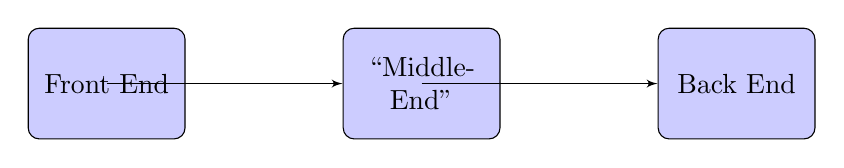
\begin{tikzpicture}[node distance = 4cm, auto]
	\node [block] (front) {Front End};
	\node [block, right of=front] (middle) {``Middle-End''};
	\node [block, right of=middle] (end) {Back End};
	
	\path [line] (front) |- (middle);
	\path [line] (middle) |- (end);
\end{tikzpicture}

\subsection{Front End}
The Front End performs lexing and parsing, which converts the set of input files into some appropriate datastructures representing the program. The lexing and parsing are implemented using fslex and fsyacc respectively, which are versions of lex and yacc ported to \fsharp. 

\subsection{Middle End}
The Middle End performs various transformations on the input data. The main three operations are \textit{lowering} various constructs to simpler ones, \textit{annotation} of the AST with additional data and \textit{checking} that the semantics of the program are correct with respect to the programming language. In order, the phases the middle end go through are as follows:\\
\begin{enumerate}
	\item{Name Lowering and Global Reference Building}
	\item{Type Parameter Annotation}
	\item{Type Expansion}
	\item{Template Expansion for Classes/Interfaces}
	\item{Building Method Maps for each Type}
	\item{Checking Interface Semantics}
	\item{Type Annotation and Template Expansion for Methods}
	\item{Fixing Function Parameters for Non-Static Methods}
\end{enumerate}

\subsection{Back End}
The Back End is entirely dedicated to code generation and the production of LLVM assembly code. The 


\section{Implementation}

\subsection{Lexing and Parsing}
The Lexing stage takes a set of input files and \textit{tokenises} them, meaning they are transformed from strings of text into tokens that are passed onto the Parsing stage.

The Parser takes the tokens and using a grammar converts these to an Abstract Syntax Tree (AST) that represents all the program structures.

\subsubsection{Abstract Syntax Tree}
The AST has 4 main components: \bcode{NamespaceDecl}s, \bcode{ClassDecl}s, \bcode{InterfaceDecl}s and \bcode{Expr}s. Each of these immutable types has a ``annotation type'' that acts as a wrapper and allows data to be attached to the declaration after it has been created by the parser. The annotation type for a particular declaration has an ``\bcode{A}'' on the end such as \bcode{NamespaceDeclA} and \bcode{ClassDeclA}.

\begin{fslisting}
type NamespaceDecl =
    | Class of Name * Visibility * IsStruct * (*interfaces*) list<PType> * list<ClassDeclA>
    | Interface of Name * Visibility * (*interfaces*) list<PType> * list<InterfaceDeclA>
   
type InterfaceDecl =
    | InterfaceProc of (*name*) Name * (*params*) list<Param> * (*returnType*) PType ref

type ClassDecl =
    | ClassVar  of Name * Visibility * IsStatic * PType ref * ExprA
    | ClassProc of Name * Visibility * IsStatic * list<Param> ref * (*returnType*) PType ref * (*body*) ExprA

type Expr =
    | ConstInt of (*size*) int * (*value*) int64
    | ConstBool of bool
    | Var of string
    | VarStatic of PType ref
    | Dot of ExprA * string
    | DotTemplate of ExprA * string * list<PType> ref
    | DotInstance of ExprA * ClassDeclA
    | DotStatic of NamespaceDeclA * ClassDeclA
    | Binop of string * ExprA * ExprA
    | Cast of PType ref * ExprA
    | Call of ExprA * list<ExprA>
    | CallStatic of ClassDeclA * list<ExprA>
    | CallInstance of ClassDeclA * ExprA * list<ExprA>
    | CallVirtual of InterfaceDeclA * ExprA * list<ExprA>
    | Assign of ExprA * ExprA
    | DeclVar of string * (*Assign*) ExprA
    | Return of ExprA
    | ReturnVoid
    | If of ExprA * ExprA * ExprA
    | While of ExprA * ExprA
    | Seq of ExprA ref * ExprA ref
    | Nop
\end{fslisting}

\subsection{Annotation/Type Annotation}

\subsection{Types}
\subsubsection{Automatic Constructors}
An automatic constructor is a shorthand to writing an explicit constructor. In the parser code in this form:
\begin{sooplisting}
class Class(x1: Type1, private x2: Type2, ..., public xN: TypeN) { /* decls */ }
\end{sooplisting}
is lowered to:
\begin{sooplisting}
class Class {
	private var x1: Type1;
	private var x2: Type2;
	// ...
	public var xN: TypeN;
	
	public static new(x1: Type1, private x2: Type2, ..., public xN: TypeN) {
		var @ret = ctor();
		@ret.x1 = x1;
		@ret.x2 = x2;
		// ...
		@ret.xN = xN;
		return @ret;
	}
	
	/* decls */
}
\end{sooplisting}

\subsection{Methods}
\subsubsection{Method Overloading/Selection}
\label{sec:methodOverloadSelection}
Lorem ipsum dolor sit amet

\subsection{Interfaces and VTables}

Multiple checks are performed on interfaces - the strongly connected components of the interface inheritance hierarchy are found using Tarjan's algorithm to see if there are any cycles - a cycle of interfaces causes an unresolvable loop to be created. Check to see whether each type implementing the interface actually implements all the interface's methods.

Interfaces allow the mechanism of dynamic dispatch which is implemented using Virtual Method Tables (VTables). Conceptually, a VTable is an array of function pointers that that each point to a particular type's implementation of a certain set of methods. At runtime, the correct implementation of a method can be determined from the type of the object being pointed to.

\subsubsection{VTable Structure}
To explain the VTable creation process, let's look at a concrete example of a \plname program:
\begin{sooplisting}
interface Vehicle {
	drive();
	getNumberOfWheels():Int8;
}

interface Flying {
	getAltitude():Int32;
}

class Car : Vehicle {
	public drive() { }
	public getNumberOfWheels():Int8 { return 4B; }
	public static new():Car { return ctor(); }
}

class Airplane : Vehicle, Flying {
	public drive() { }
	public getNumberOfWheels():Int8 { return 2B; }
	public getAltitude():Int32 { return 42000; }
}
\end{sooplisting}
The process advances as follows:
\begin{enumerate}
	\item{
		Each interface method is given a unique id.
		
	}
	\item{
		A \bcode{VTable} type is created - it is a struct containing a function pointer for each interface method (ordered according to their id).
		\begin{llvmlisting}
%VTable = type { i32 (%Interface*)*, void (%Interface*)*, i8 (%Interface*)* }
		\end{llvmlisting}
	}
	\item{
		For each type $T$ an instance of the \bcode{VTable} is instantiated - for each interface method $T$ implements, a function pointer to $T$'s method implementation is put into the \bcode{VTable}.
		\begin{llvmlisting}
@VTable___T__Airplane = global %VTable {
	i32 (%Interface*)* @"T::Airplane.getAltitude+Stub", 
	void (%Interface*)* @"T::Airplane.drive+Stub", 
	i8 (%Interface*)* @"T::Airplane.getNumberOfWheels+Stub" }
@VTable___T__Car = global %VTable { 
	i32 (%Interface*)* null,
	void (%Interface*)* @"T::Car.drive+Stub",
	i8 (%Interface*)* @"T::Car.getNumberOfWheels+Stub" }
		\end{llvmlisting}
	}
	\item {
		Stub methods are created into order to keep using (and so take advantage of) LLVM's strong type system. They cast the generic \bcode{\%Interface} type to the concrete type and call the original method. There is no overhead from these extra function calls as they be inlined by the LLVM optimiser.
		\begin{llvmlisting}
define i32 @"T::Airplane.getAltitude+Stub"(%Interface* %this) {
entry:
  %0 = bitcast %Interface* %this to %T__Airplane*
  %1 = call i32 @T__Airplane.getAltitude(%T__Airplane* %0)
  ret i32 %1
}
		\end{llvmlisting}
	}
	\item{
		The concrete types are then constructed, each with a pointer to it's VTable as the first field.
		\begin{llvmlisting}
%T__Airplane = type { %VTable* }
%T__Car = type { %VTable* }
%Interface = type { %VTable* }
		\end{llvmlisting}
	}
\end{enumerate}
Graphically, the layout of the LLVM types can be presented as:\\
% http://tex.stackexchange.com/questions/40128/creating-process-table-figure-in-tikz
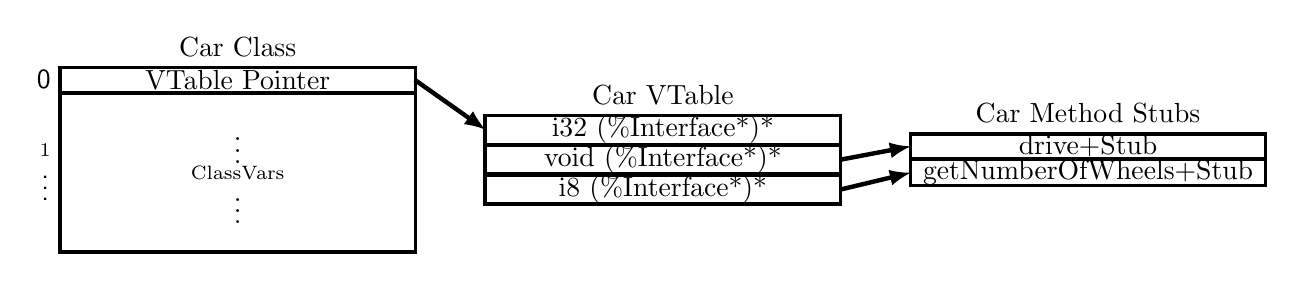
\begin{tikzpicture}
\matrix (class) at (0,0) [table matrix,label={[align=center]90:{Car Class}}]
{
VTable Pointer\\
|[minimum height=2cm]| $\substack{\vdots\\ \mathrm{Class Vars}\\ \vdots}$\\
};

\matrix (vtable) at (5.4,0) [table matrix,label={[align=center]90:{Car VTable}}]
{
i32 (\%Interface*)*\\
void (\%Interface*)*\\
%|[minimum height=2.5cm]| $\vdots$\\
i8 (\%Interface*)*\\
};

\matrix (stubs) at (10.8,0) [table matrix,label={[align=center]90:{Car Method Stubs}}]
{
drive+Stub\\
getNumberOfWheels+Stub\\
};

\foreach \x/\y in {1/0,2/$\substack{1\\ \vdots}$} {
	\node[anchor=east] at (class-\x-1.west) {\textsf{\y}};
}
\draw[black,-latex,ultra thick] (class-1-1.east) -- (vtable-1-1.west);
\draw[black,-latex,ultra thick] (vtable-2-1.east) -- (stubs-1-1.west);
\draw[black,-latex,ultra thick] (vtable-3-1.east) -- (stubs-2-1.west);
\end{tikzpicture}

\subsubsection{Virtual Method Call}
Following one from the previous example, let's see what would happen if we were to perform a virtual method call on the \bcode{drive} method of a \bcode{Vehicle}:
\begin{sooplisting}
var v = (Vehicle) Car.new();
v.drive();
\end{sooplisting}
Focusing on the \bcode{v.drive()} statement, assuming \bcode{\%v} is the a pointer to the value of \bcode{v}:
\begin{enumerate}
	\item{
		Load the reference to \bcode{v} into \bcode{\%v1}.
		\begin{llvmlisting}
%v1 = load %Interface** %v
		\end{llvmlisting}
	}
	\item{
		Load the pointer to \bcode{Car}'s 0th element (its VTable) into \bcode{\%3}.
		\begin{llvmlisting}
%2 = getelementptr inbounds %Interface* %v1, i32 0, i32 0
%3 = load %VTable** %2
		\end{llvmlisting}
	}
	\item{
		Load the VTable's 1st element (its function pointer for \bcode{Vehicle.drive}) into \bcode{\%5}.
		\begin{llvmlisting}
%4 = getelementptr inbounds %VTable* %3, i32 0, i32 1
%5 = load void (%Interface*)** %4
		\end{llvmlisting}
	}
	\item{
		Call the function, passing the reference to \bcode{v} as the \bcode{this} parameter.
		\begin{llvmlisting}
call void %5(%Interface* %v1)
		\end{llvmlisting}
	}
\end{enumerate}


\subsection{Mixins and Inheritance}
Once all the lowering operations have completed, the only datatypes left in the language are \textit{classes}, \textit{structs}, \textit{interfaces}. Mixins in \plname are similar to \textit{abstract classes} in object oriented programming languages such as Java. They are the main unit of code reuse and also allow multiple inheritance but without the usual problems such as the Diamond Problem. They are implemented as structs that can only be instantiated from a mixin statement. A mixin statement is similar to a \bcode{private val} statement. A mixin \bcode{Foo} automatically creates an interface of the same name.
\begin{sooplisting}
mixin 
\end{sooplisting}

\subsection{Binary Operators}
Binary operators are defined as \bcode{public static} methods that use symbols instead of names and have precisely two parameters. In the \textit{Binop Lowering Phase}, a list $L$ of every binary operator is compiled by searching each class for all the methods that fit this definition. For each \bcode{Binop (name, left, right)} expression in the AST, the best overload $M$ from $L$ fitting the \bcode{name} and types of \bcode{left} and \bcode{right} is selected and the \bcode{Binop} expression is replaced by a static call to $M$. For example, using the following binary operator definition: 
\begin{sooplisting}
class Operators {
	public static **(a: Int32, b: Int32): Int32 {
		return a * a + b * b;	
	}
}
\end{sooplisting}
The AST of the following expression:
\begin{sooplisting}
1 ** 3; // Binop (Var "**", ConstInt (32, 1), ConstInt (32, 3))
\end{sooplisting}
Will be changed into an AST that would be created from the following equivalent code:
\begin{sooplisting}
Operators.**(1, 3);
// Call (Dot (VarStatic "Operators", "**")), [ConstInt (32, 1), ConstInt (32, 1)]
\end{sooplisting}

\subsubsection{Precedence}
The binary operator precedence is defined similar to FSharp -- the first character of the operator determines its precedence from the table below. When an operator of precedence level $p$ is lexed, a token of the form \bcode{BINOP$p$} is created; in fsyacc (the parsing stage) the tokens \bcode{BINOP$p$} for $p=1,2,\dots,6$ have their precedence defined by the \bcode{\%left} instruction.
\begin{center}
\begin{tabular}{ | c | c | }
\hline
Operator Character & Precedence \\ \hline
* / & 6 \\ \hline
\% & 5 \\ \hline
+ $-$ & 4 \\ \hline
= < > & 3 \\ \hline
? ! & 2 \\ \hline
\& & 1 \\ \hline
| & 0 \\ \hline
\end{tabular}
\end{center}
Special treatment is given to the \bcode{\&\&} and \bcode{||} operators so that they short circuit. 
\subsection{Arrays}
$a[i]$ gets changed to a.indexer(i)\\
$a[x_1][x_2]\dots[x_n] = v$ is lowered to \code{a.indexer($x_1$).indexer($x_2$)}$\dots$\code{.indexer($x_n$,$v$)}

\subsection{Templates}
Templates provide \textit{parametric polymorphism} to data types and methods whilst preserving the static type-safety of the language. They perform a similar purpose to generics in \csharp and Java, have a similar syntax to templates in D but are implemented in much the same as \cpp templates (except they lack the ability to use integral data types as template parameters or any kind of template specialisation).

\subsubsection{Syntax}
The syntax for templates in \plname differs from the most other implementations -- the form \bcode{TypeName<T1,T2,$\dots$,Tn>} is used by \csharp, Java, \cpp and many others but leads to ambiguities when lexing and parsing. When used with the standard binary operators \bcode{<}, \bcode{>} and function calls using parentheses and commas, the expression \bcode{foo(TypeName<A,B>.bar)} cannot be parsed with an LR(1) parser. Ambiguity arises when the parsing automaton reaches the comma - without looking ahead at least 3 tokens (and seeing the full stop) and it cannot decide whether the statment should be parsed as \bcode{foo(TypeName is less than A,$\dots$)} or \bcode{foo(TypeName with generic parameters A,$\dots$)}. Lexing is also a problem as the operator \bcode{>>} is often used as the right bitshift operator which can cause issues in types with nested template parameters like \bcode{Box<Box<Int32>>}.

\plname avoids these problems by using the unambiguous form \bcode{TypeName`[T1,T2,$\dots$,Tn]} where $T1 \dots Tn$ are the \textit{type parameters}.
\begin{sooplisting}
class Box`[T] {
	private var item: T;
	
	public static new(item: T):Box`[T] {
		var b = ctor();
		b.item = item;
		return b;
	}
	
	public getItem():T { return item; }
}
\end{sooplisting}

\subsubsection{Template Expansion}
Template expansion takes place in two stages: in the first stage, called \textit{Template Type Expansion}, parametrised data types are expanded; in the second stage, called \textit{Template Method Expansion} parametrised methods are expanded. 

\paragraph{Template Type Expansion}
A depth first search is performed on the AST with the non-template data types as roots. The program descends the AST and for each template declaration of a template type it checks if it has already been found, if not it clones the template type replacing the type parameters. The listing below shows the possible places that a template can be instantiated once all constructs have been lowered to the base classes/structs and interfaces.
\begin{sooplisting}
class Class`[...] : ~~IFace1`[...]~~,...,~~IFaceN`[...]~~ {

	public method`[...](t1: ~~Type1`[...]~~, ..., tN: ~~TypeN`[...]~~):~~Type`[...]~~ {
		[~~CastType[...]~~] castExpr;
		var foo = ~~VarStaticType[...]~~.dotName;
	}	
	private var variable: ~~Type`[...]~~;
}

interface IFace`[...] : ~~IFace1`[...]~~,...,~~IFaceN`[...]~~ {
	public method`[...](t1: ~~Type1`[...]~~, ..., tN: ~~TypeN`[...]~~):~~Type`[...]~~;
}
\end{sooplisting}

\paragraph{Template Method Expansion}
Methods cannot be expanded until the \textit{Type Annotation Phase} as the types of the calling arguments must be known in order to select the correct overload. For example, on a class \bcode{Foo} there may exist static methods \bcode{bar`[T](a:Bool, b:T)} and \bcode{bar`[T](a:Int32, b:T)} -- which template method is expanded for a call of \bcode{Foo.bar`[Int32](v,0)} where \bcode{v} is a variable depends on the type of \bcode{v}. Similarly, for \bcode{a.foo`[Type]()} the type of \bcode{a} must be known to determine which datatype to expand \bcode{foo} in.\\\\
For example, take the following piece of code that causes template method expansion for a static call:
\begin{sooplisting}
class Program {
	public static id`[A](a: A, b: Int32):A { return a; }
	public static id`[A](a: A, b: Bool):A  { return a; }
	public static id`[A,B](a: A, a:B):A    { return a; }

	public static main() {
		Program.id`[Int32](3,true);
	}
}
\end{sooplisting}
The algorithm to expand the templates proceeds as follows:
\begin{enumerate}
	\item{In an expression (\bcode{main()}) a parametrised static call $c$ (\bcode{Program.id`[Int32](3,true)}) is found}.
	\item{The set of methods signatures $M$ in the target type $T$ (\bcode{Program}) that are static and have the same name (\bcode{id}), number of type parameters (1) and number of formal parameters (2) as $c$ is constructed ($\{\bcode{id`[A](A,Int32)}, \bcode{id`[A](A,Bool)}\}$).}
	\item{Template expansion is performed on each signature $m \in M$ in isolation, returning a set of expanded methods signatures $M'$ ($\{\bcode{id(Int32,Int32)}, \bcode{id(Int32,Bool)}\}$).}
	\item{Out of $M'$ the appropriate expanded overload $m'$ is selected (\bcode{id(Int32,Bool)} using the process described in section \ref{sec:methodOverloadSelection}).}
	\item{The method that expanded out to have signature $m'$ is fully expanded and added to $T$.}
\end{enumerate}
Instance calls cause expansion in the same way only with $T$ differing and performing the search for instance rather than static methods. 


\subsubsection{Example LLVM Output}

\subsection{Memory Allocation and Garbage Collection}
Currently, \bcode{malloc} is used for memory allocation and memory is never freed. The Boehm Conservative Collector could easily be linked to the output of the program and calls to \bcode{malloc} replaced with calls to \bcode{GC\_MALLOC} and a garbage collector would be enabled.

\printbibliography

\end{document}





















































